\chapter{Station B: Tatort Konto}\label{ch:tatort_konto}

\begin{myremark}
	Jemand hat Lenas Konto übernommen. Lena ist sicher: \enquote{Mein Passwort kennt niemand!}
	An dieser Station finden Sie heraus, wie Angreiferinnen und Angreifer trotzdem an Passwörter kommen -- und wie Sie sich schützen.
\end{myremark}

\section{Drei Wege zu fremden Passwörtern}

\begin{mysummary}
	\begin{enumerate}
		\item \textbf{Ausprobieren:} Ein Computer probiert automatisch sehr viele Passwörter durch. Zuerst bekannte Passwörter und Wörter aus dem Wörterbuch, dann alle möglichen Kombinationen.
		\item \textbf{Datenleck:} Eine Webseite wird gehackt und die Passwörter werden veröffentlicht. Wer überall dasselbe Passwort nutzt, verliert so alle Konten auf einmal.
		\item \textbf{Phishing:} Eine gefälschte Nachricht lockt auf eine gefälschte Login-Seite. Man gibt das Passwort freiwillig ein -- direkt an die Betrüger.
	\end{enumerate}
\end{mysummary}

\section{Wie lange dauert das Ausprobieren?}

Ein leistungsstarker Computer kann bei einem gestohlenen Passwortspeicher etwa \tib{10 Milliarden} ($10^{10}$) Passwörter pro Sekunde ausprobieren.
Wie viele Möglichkeiten es gibt, hängt vom \tib{Zeichenvorrat} (wie viele verschiedene Zeichen) und der \tib{Länge} ab:
Bei 26 Kleinbuchstaben und Länge 6 gibt es $26 \cdot 26 \cdot 26 \cdot 26 \cdot 26 \cdot 26 = 26^6$ Möglichkeiten.

\begin{myexercise}[Passwörter knacken -- nachgerechnet]\label{ex:passwort_rechnen}
	Ergänzen Sie die Tabelle mit dem Taschenrechner. Die erste Zeile ist als Beispiel ausgefüllt.
	Rechnen Sie die Zeit in eine anschauliche Einheit um (Sekunden, Stunden, Tage, Jahre).

	\begin{center}
		\renewcommand{\arraystretch}{1.6}
		\begin{tabular}{p{4.4cm}ccp{2.4cm}p{2.6cm}}
			\textbf{Passwort-Art}             & \textbf{Vorrat} & \textbf{Länge} & \textbf{Möglichkeiten}  & \textbf{Zeit}         \\
			\midrule
			nur Kleinbuchstaben               & 26              & 6              & $26^6 \approx \num{3.1e8}$ & \num{0.03}~s        \\
			nur Kleinbuchstaben               & 26              & 8              &                         &                       \\
			Klein-, Grossbuchstaben, Ziffern  & 62              & 8              &                         &                       \\
			Klein-, Grossbuchstaben, Ziffern  & 62              & 12             &                         &                       \\
			4 zufällige Wörter aus einer Liste & 7776           & 4              &                         &                       \\
			5 zufällige Wörter aus einer Liste & 7776           & 5              &                         &                       \\
		\end{tabular}
	\end{center}

	Was hilft mehr: ein grösserer Zeichenvorrat oder eine grössere Länge? Begründen Sie mit der Tabelle.
	\schreibzeile

	\begin{myanswer}
		\begin{tabular}{lll}
			26, Länge 8:   & $\approx \num{2.1e11}$ & ca. 21~s               \\
			62, Länge 8:   & $\approx \num{2.2e14}$ & ca. 6~Stunden           \\
			62, Länge 12:  & $\approx \num{3.2e21}$ & ca. \num{10000}~Jahre   \\
			4 Wörter:      & $\approx \num{3.7e15}$ & ca. 4~Tage              \\
			5 Wörter:      & $\approx \num{2.8e19}$ & ca. 90~Jahre            \\
		\end{tabular}

		Die Länge hilft am meisten, weil sie im Exponenten steht: Jedes zusätzliche Zeichen vervielfacht die Anzahl Möglichkeiten.
		Wichtig: Diese Zeiten gelten nur für \emph{zufällige} Passwörter. Bekannte Wörter, Namen oder Muster wie \enquote{Hund2024!} werden mit Wörterlisten fast sofort gefunden.
	\end{myanswer}
\end{myexercise}

\section{Ein gutes Passwort bauen}

\begin{myprocedure}[Zwei Methoden für starke Passwörter]
	\begin{itemize}
		\item \textbf{Wörter-Methode:} Wählen Sie vier oder fünf \emph{zufällige} Wörter, die nichts miteinander zu tun haben, z.\,B. \enquote{Kaktus Wolke Trompete Senf Igel}.
		      Lang, aber gut zu merken.
		\item \textbf{Satz-Methode:} Denken Sie sich einen Satz aus und nehmen Sie die Anfangsbuchstaben, Zahlen und Satzzeichen:
		      \enquote{Am Montag esse ich 2 Gipfeli und trinke 1 Kakao!} wird zu \enquote{AMei2Gut1K!}.
	\end{itemize}
	Für jedes Konto ein anderes Passwort -- dabei hilft ein \tib{Passwortmanager}, der alle Passwörter sicher speichert.
\end{myprocedure}

\begin{myexercise}[Passwort-Test]
	\begin{enumerate}
		\item Bilden Sie mit jeder Methode ein \emph{Beispiel}-Passwort, das Sie nirgends verwenden.
		\item Testen Sie Ihre Beispiele und zum Vergleich \enquote{Lena2013} auf der Seite\\
		      \url{https://www.passwortcheck.ch} (ein Angebot der Daten\-schutz\-beauf\-trag\-ten des Kantons Zürich). Notieren Sie die Ergebnisse.
	\end{enumerate}
	\schreibzeile
	\schreibzeile
\end{myexercise}

\begin{myexercise}[Lenas Fehler]
	Lena hatte für ihr Social-Media-Konto dasselbe Passwort wie für ein Gaming-Forum.
	Letzten Monat wurde dieses Forum gehackt und die Liste der Benutzernamen und Passwörter im Internet veröffentlicht.
	Erklären Sie, wie die Angreifer so an Lenas Social-Media-Konto kamen, und nennen Sie zwei Massnahmen, die das verhindert hätten.
	\schreibzeile
	\schreibzeile
	\schreibzeile
	\begin{myanswer}
		Angreifer probieren veröffentlichte Kombinationen aus Benutzername (oder E-Mail) und Passwort automatisch bei anderen Diensten aus.
		Weil Lena das Passwort wiederverwendet hat, funktionierte es auch bei ihrem Social-Media-Konto.
		Massnahmen: für jedes Konto ein eigenes Passwort (Passwortmanager); \gls{TFA} einschalten.
	\end{myanswer}
\end{myexercise}

\section{Der zweite Schlüssel}

Bei der \tib{Zwei-Faktor-Authentifizierung} (\acrshort{TFA}) braucht es für die Anmeldung zwei verschiedene Dinge:
etwas, das Sie \emph{wissen} (Passwort), und etwas, das Sie \emph{haben} (Handy mit Code-App oder SMS-Code).
Selbst wer Ihr Passwort kennt, kommt ohne Ihr Handy nicht in Ihr Konto.

\begin{myexercise}[Habe ich einen zweiten Schlüssel?]
	Finden Sie bei einer App oder einem Konto, das Sie nutzen, die Einstellung für die \gls{TFA}
	(oft unter \enquote{Sicherheit}, \enquote{Anmeldung} oder \enquote{Konto}). Ist sie eingeschaltet?
	Notieren Sie den Weg. Aktivieren Sie sie, wenn Sie möchten -- bei Unsicherheit zusammen mit Ihren Eltern.
	\schreibzeile
\end{myexercise}

\section{Phishing-Detektiv}

Phishing-Nachrichten wirken oft echt. Seit es \gls{KI} gibt, sind sie sogar fehlerfrei und persönlich formuliert.
Achten Sie deshalb weniger auf Rechtschreibfehler, sondern auf diese \tib{Warnsignale}:
Zeitdruck oder Drohung, ungewöhnliche Bitte (Geld, Passwort, Code), unbekannter Absender, Link mit seltsamer Adresse, \enquote{zu gut, um wahr zu sein}.

\begin{myexercise}[Echt oder Falle?]\label{ex:phishing}
	Entscheiden Sie bei jeder Nachricht: echt oder Falle? Notieren Sie die Warnsignale in der Tabelle. Alle Firmen, Adressen und Nummern sind erfunden.

	\begin{center}
		\begin{tabular}{ccc}
			\textbf{(a)} SMS & \textbf{(b)} Mitteilung & \textbf{(c)} Chat \\
			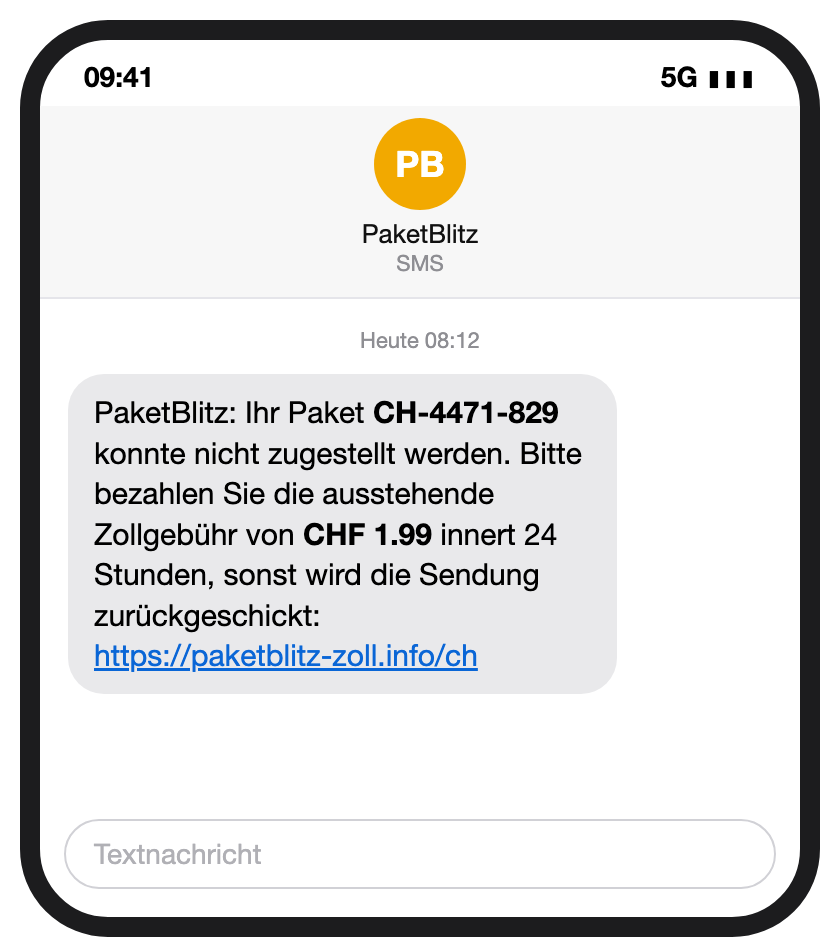
\includegraphics[height=5.4cm,keepaspectratio]{Medienkompetenzwoche/UG_Datenschutz/Figures/1_sms_paketblitz} &
			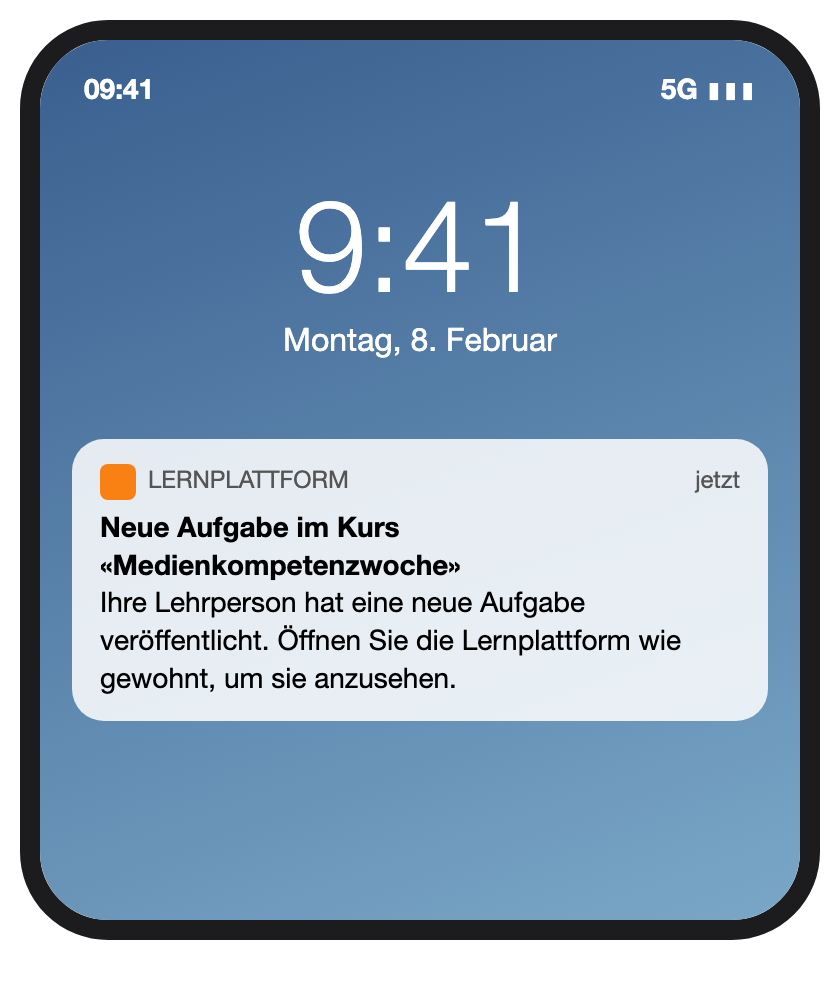
\includegraphics[height=5.4cm,keepaspectratio]{Medienkompetenzwoche/UG_Datenschutz/Figures/3_push_lernplattform} &
			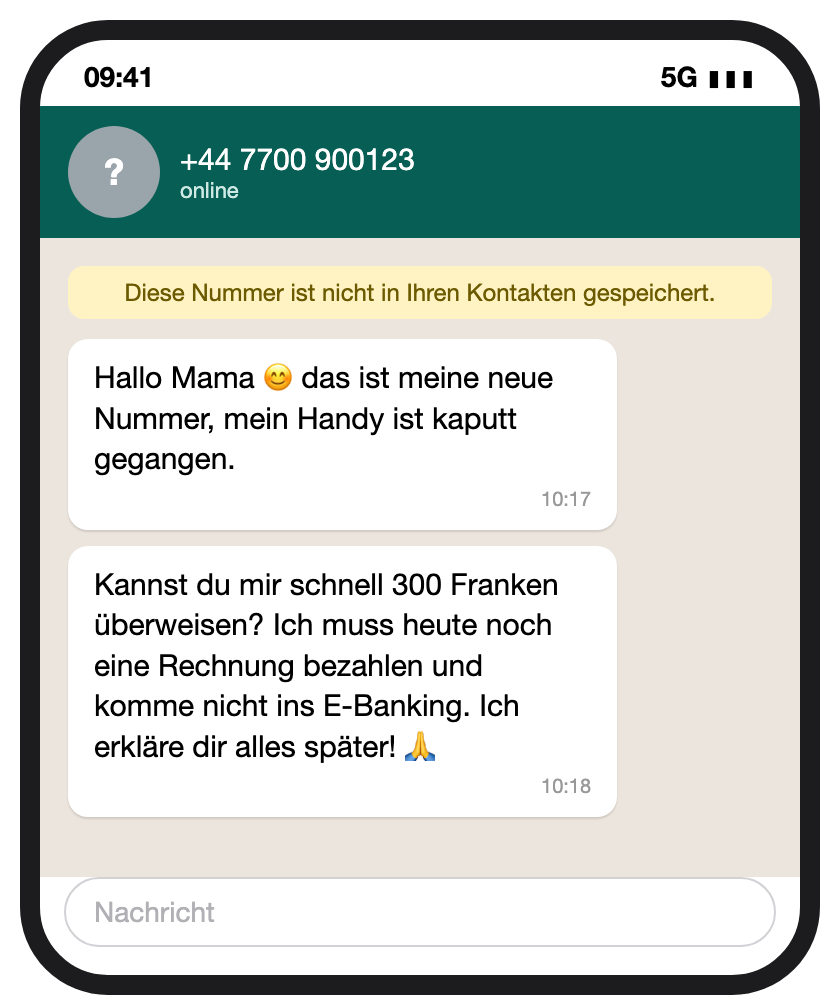
\includegraphics[height=5.4cm,keepaspectratio]{Medienkompetenzwoche/UG_Datenschutz/Figures/4_chat_hallomama} \\[3mm]
		\end{tabular}

		\textbf{(d)} E-Mail\\[1mm]
		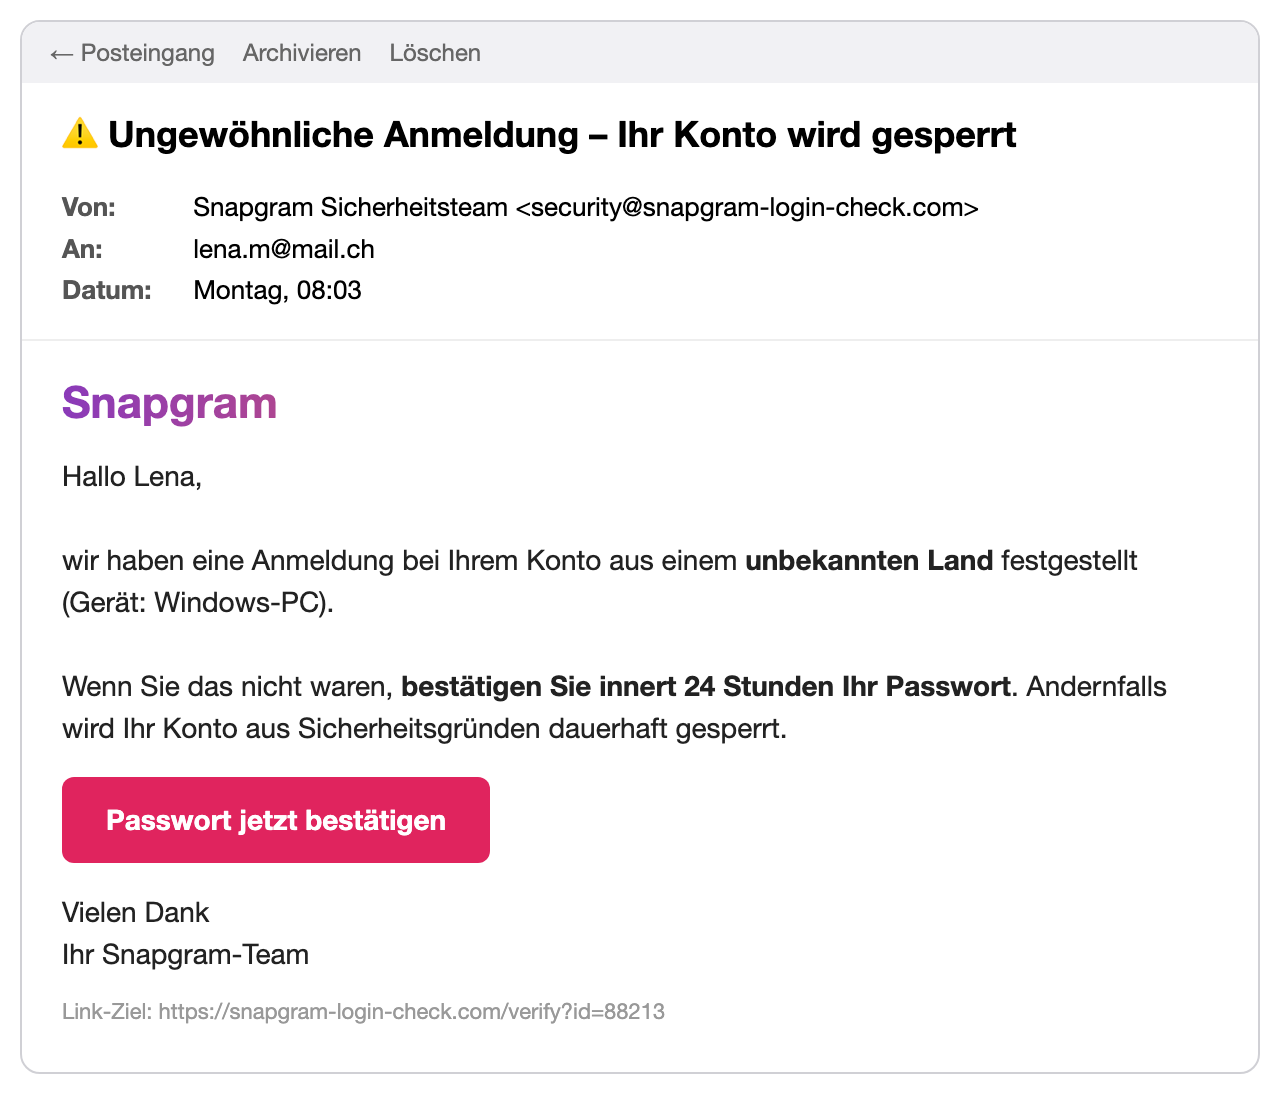
\includegraphics[width=0.72\linewidth,keepaspectratio]{Medienkompetenzwoche/UG_Datenschutz/Figures/2_mail_snapgram}
	\end{center}

	\begin{center}
		\renewcommand{\arraystretch}{1.5}
		\begin{tabular}{p{0.8cm}p{2.6cm}p{9cm}}
			\textbf{Nr.} & \textbf{echt / Falle} & \textbf{Warnsignale}  \\
			\midrule
			(a)          &                       &                       \\
			(b)          &                       &                       \\
			(c)          &                       &                       \\
			(d)          &                       &                       \\
		\end{tabular}
	\end{center}

	\begin{myanswer}
		\begin{aenum}
			\item Falle: Zeitdruck, kleiner Betrag als Köder (es geht um die Kreditkartendaten), fremde Internetadresse.
			\item Wahrscheinlich echt: kein Link, keine Bitte um Daten, man soll die Plattform \enquote{wie gewohnt} öffnen. Trotzdem gilt: nie über Links in Nachrichten anmelden.
			\item Falle (\enquote{Hallo-Mama}-Betrug): unbekannte (ausländische) Nummer, Geldforderung, Zeitdruck. Immer über die bekannte Nummer zurückrufen.
			\item Falle: Drohung (Sperrung), Zeitdruck, Aufforderung zur Passworteingabe; die Adressen von Absender und Link gehören nicht zum echten Dienst.
		\end{aenum}
	\end{myanswer}
\end{myexercise}

\begin{mychallenge}[Phishing-Quiz]
	Machen Sie das Phishing-Quiz unter \url{https://phishingquiz.withgoogle.com}. Name und E-Mail-Adresse dürfen Sie erfinden.
	Wie viele von acht Nachrichten haben Sie richtig erkannt? Welches Warnsignal hatten Sie übersehen?
	\schreibzeile
\end{mychallenge}

\begin{fallakte}[-- Station B]
	Wie kamen die Angreifer an Lenas Konto? Was hätte sie anders machen können?
	\schreibzeile
	\schreibzeile
	\schreibzeile
\end{fallakte}
